\chapter{Background and Literature Review}
\label{ch:bg-lit}
This chapter establishes the municipal, empirical and technical foundations of the dissertation. It first defines municipal visual monitoring in the Maltese context and introduces the \gls{MDWD} and \gls{MTSD}, comparing them with related datasets in the literature. It then reviews the \gls{CV} tasks and model paradigms used in the empirical work, before concluding with the deployment and evaluation concepts relevant to the study.

\section{Municipal Visual Monitoring}
\label{sec:bg-municipal}
Municipal visual monitoring refers to the repeated observation of public spaces and infrastructure in order to identify conditions that may require cleansing, maintenance or further attention \cite{torneiro2025urbanmonitoring}. This formulation underpins both kerbside waste and roadside infrastructure as monitoring domains, and is shaped in turn by the characteristics of the Maltese setting in which it is applied.

\subsection{Municipal Monitoring and Visual Observation}
\label{sec:bg-municipal-inspection}
Municipal monitoring conventionally relies on observations of the physical environment, obtained through routine inspections by municipal personnel and reports submitted by members of the public \cite{BG1-repeatedinspection,BG2-waste-reporting,BG3-citizen-reporting}. Human assessment remains important, since the significance of an observed condition often depends on contextual and operational knowledge that extends beyond its visual appearance \cite{BG4-human-inspection}. Automated visual monitoring is accordingly treated here as a means of supporting existing inspection and reporting practice, extending its coverage rather than substituting for the contextual judgement on which operational decisions depend.

Within this dissertation, a municipal visual observation is understood to accumulate information across successive stages. An object of interest is first identified within the streetscape and spatially localised, after which it is characterised according to properties relevant to the corresponding municipal service. Where imagery is associated with geographical position, the resulting observation can additionally be linked to the location at which the condition was encountered, giving it both a description and a place within the road network.

Opportunistically captured imagery, gathered during journeys undertaken for other purposes, extends observation beyond dedicated inspection activity and increases the spatial frequency at which municipal conditions are encountered \cite{BG7-driveby-sensing,BG10-vehicle-sensing}. Such imagery can be processed automatically, with selected observations flagged for review so that subsequent inspection effort is concentrated where conditions are more likely to warrant it.

\subsection{Waste and Road Infrastructure as Monitoring Domains}
\label{sec:bg-monitoring-domains}
As established in Section~\ref{sec:problem-definition}, this dissertation considers two municipal monitoring domains, namely kerbside domestic waste and traffic-sign infrastructure, whose operational characteristics differ substantially. Waste represents a comparatively transient condition whose presence, presentation and relevance may change between successive collection cycles \cite{wastecollection2026web,era2023web}, whereas traffic signs and related roadside infrastructure are persistent physical assets whose state changes more gradually through ageing, damage and environmental exposure \cite{BG14-sign-degradation,BG5-sign-monitoring}. Despite this distinction, both can be expressed through a common visual-monitoring formulation in which relevant objects are first localised within street-level imagery and subsequently characterised using information meaningful to the responsible service.

For kerbside waste, characterisation extends beyond establishing that discarded material is present. Waste encountered within the streetscape may include standard collection bags, loose discarded objects, bulky items and material associated with \gls{CMD}'s cleansing activities \cite{BG15-mdwd,wasteserv2026web}. Its interpretation depends partly on presentation, since the Maltese collection system associates different domestic waste streams with designated formats and collection schedules \cite{wastecollection2026web,era2023web}. Distinguishing these visually observable streams therefore provides information a single generic waste category would not capture, motivating the categories defined for the \gls{MDWD} in Subsection~\ref{sec:bg-mdwd}.

Road-infrastructure monitoring similarly extends beyond recognising the semantic category of a traffic sign. Conventional sign recognition is principally concerned with recovering the regulatory or informational meaning conveyed by the sign face, whereas infrastructure monitoring is also concerned with the physical asset through which that meaning is displayed. Properties such as mounting configuration, viewing orientation and visible physical condition therefore remain relevant even when semantic identity is uncertain \cite{BG16-malta-sign-guidelines,BG16-eu-rism,BG29-sign-inspection}. Deterioration, including fading, surface damage and loss of visibility, may affect whether an asset requires inspection or maintenance \cite{BG14-sign-degradation,BG5-sign-monitoring}, and a rear-facing or otherwise unidentifiable sign can likewise remain a useful infrastructure observation even when its meaning cannot be recovered from the available image. These requirements motivate the object and attribute taxonomy adopted for the \gls{MTSD}, described in Subsection~\ref{sec:bg-mtsd}.

The two domains therefore diverge in what gives an observation its significance: the transient presentation of waste, as against the persistent identity, installation and physical state of infrastructure. In both cases, however, localisation alone provides an incomplete observation. It is the combination of location and domain-specific characterisation that forms the common basis for the two monitoring problems considered in this dissertation.

\subsection{The Maltese Streetscape and Monitoring Environment}
\label{sec:bg-malta}
Both monitoring domains are additionally shaped by the environment in which they are observed. Malta combines high population density and extensive urban development within a small and strongly car-dependent island state, where limited street space is divided between vehicular movement, parking, pedestrians, building frontages and roadside infrastructure \cite{I5-malta,I6-malta,BG19-malta-slow-streets}. Many localities contain narrow streets and pavements together with substantial on-street parking, restricting sightlines towards objects positioned close to the kerb and increasing the likelihood of partial occlusion by vehicles and surrounding street furniture \cite{BG18-malta-walkability,BG15-mdwd}.

Each domain introduces its own locally specific source of visual variation. Domestic waste streams are collected through a national door-to-door system in which waste is placed at the kerbside in designated colour-coded bags on scheduled collection days, appearing directly within the public streetscape, commonly at pavement or kerb level and alongside parked vehicles and other visually competing objects \cite{wastecollection2026web,era2023web,BG15-mdwd}. Colour and presentation therefore provide visually observable information directly related to the collection system within which waste is encountered. Traffic-sign infrastructure, by contrast, is shaped primarily by structural rather than presentational differences. Maltese specifications for permanent roadside signs encompass multiple configurations and requirements for sign plates, retro-reflective materials, supporting structures and mounting hardware \cite{infrastructuremalta2020spec}, so that roadside assets vary in semantic function, geometric form, orientation and mounting configuration, often positioned close to buildings, boundary walls and utility poles within a constrained streetscape.

Image acquisition and environmental exposure introduce additional sources of inconsistency. Street-level imagery may exhibit substantial contrast between direct sunlight and shadow, glare can obscure otherwise visible sign surfaces, and movement of the capturing platform can introduce blur \cite{BG15-mdwd,BG20-sign-glare}. Malta's marine environment is also significant over the longer term, since exposure to marine atmospheres can accelerate corrosion of metallic components, while traffic-sign retro-reflectivity and surface condition deteriorate progressively through service life \cite{BG21-marine-corrosion,BG14-sign-degradation}. This deterioration occurs along a continuum rather than as an immediate transition between an intact and failed state, supporting the use of ordered visual categories to describe physical condition \cite{BG22-sign-condition}. These characteristics collectively motivate the use of locally representative imagery when evaluating municipal visual monitoring within the Maltese streetscape.

\newpage
\subsection{Governance and Operational Responsibility}
\label{sec:bg-governance}
These environmental and structural characteristics are compounded by the distribution of institutional responsibility for the two domains across several Maltese public bodies. Kerbside domestic waste collection is organised through local and regional councils under the national collection framework, WasteServ Malta operates downstream treatment and disposal facilities, and the \gls{CMD} handles public cleansing and the removal of illegally deposited waste \cite{wastecollection2026web,era2023web,wasteserv2026web,cmd2026web}. Transport Malta provides national transport regulation and traffic-sign guidance, Infrastructure Malta develops and maintains substantial parts of the road network, and local councils retain authority over roads and public spaces within their respective localities \cite{transportmalta2021guidelines,infrastructuremalta2020spec,localcouncilsact1993}.

This distribution gives geographical position a further operational role beyond that already established for object identity and condition, since the appropriate destination of an observation can depend on where it was captured as much as what it describes. Within the Maltese setting, this reinforces the case for locally representative data and for the richer, object-level descriptions adopted by the two datasets introduced in Section~\ref{sec:bg-datasets}.

\section{Datasets and Annotation Taxonomies}
\label{sec:bg-datasets}
The two monitoring domains established in Subsection~\ref{sec:bg-monitoring-domains} are represented through two purpose-built Maltese datasets, whose object categories and attributes define the corresponding municipal observations as annotated \gls{CV} tasks. The \gls{MDWD} describes kerbside domestic waste primarily through visible presentation, while the \gls{MTSD} combines roadside-asset categories with object-level attributes describing viewing angle, mounting type, physical condition and geometric shape. Their construction, annotation procedures and \gls{EDA} are detailed in Section~\ref{sec:md-dataset-construction}.

\glsreset{MDWD}
\glsreset{MTSD}
\subsection{\gls{MDWD}}
\label{sec:bg-mdwd}
The \gls{MDWD} is a street-level \gls{OD} dataset developed to represent \gls{MSW} as it is visually encountered within the Maltese streetscape \cite{BG15-mdwd}. Its five object classes distinguish the principal bag-based streams of the national kerbside collection system from waste associated with public cleansing and other forms of waste that fall outside these streams \cite{BG15-mdwd,wastecollection2026web}. The taxonomy is based on characteristics that can be determined from road-facing imagery, primarily presentation, colour, form and context, rather than on the underlying material composition of an object. This is necessary because the contents of sealed or opaque refuse bags cannot be determined visually, and assigning labels based on information unavailable in the image would introduce systematic annotation uncertainty.

\subsubsection{Waste Terminology and Annotation Scope}
\label{sec:bg-waste-term}
The terminology used for waste requires separating the physical object being observed from the circumstances under which it entered the streetscape. In its broadest sense, \emph{waste} follows the definition established by the European Union Waste Framework Directive as a substance or object that its holder discards, intends to discard, or is required to discard \cite{BG23-waste-framework}. Within this category, \emph{kerbside-presented \gls{MSW}} is used throughout this dissertation for domestic waste intentionally placed for collection under the established national schedule \cite{wastecollection2026web}.

\emph{Litter} instead refers to loose waste whose visible presentation is consistent with material having been dropped, left or deposited in a public place rather than presented for scheduled collection. This follows the distinction in Maltese legislation between litter deposited in public spaces and refuse lawfully presented for collection \cite{BG24-malta-litter}. A related but separate category, \emph{bulky waste}, describes large discarded objects such as furniture, mattresses and household appliances \cite{BG25-bulky-waste}. By contrast, \emph{illegal dumping} describes the circumstances and legality of disposal rather than a category defined by visual appearance \cite{BG26-illegal-disposal}.

What separates kerbside-presented waste, litter and illegal dumping from one another is therefore largely a matter of intent and legality rather than appearance: a black bag placed at the kerb on collection day and one dumped illegally elsewhere may be visually indistinguishable, yet correspond to entirely different operational categories. Bulky waste, by contrast, is defined by the physical form of the object itself, and may co-occur with any of these circumstances. As intent, legality and circumstance cannot reliably be recovered from an image, the taxonomy set out below instead classifies instances according to the collection stream that their presentation most plausibly indicates, rather than by the terminology introduced above.

\subsubsection{Object-Class Taxonomy}
\label{sec:bg-mdwd-taxonomy}
The five \gls{MDWD} classes are summarised in Table~\ref{tab:mdwd-taxonomy}. For the principal streams, the operational meaning of each class is defined by the national collection scheme \cite{wastecollection2026web,era2023web}, while annotation follows the bag type visible within the image.

\begin{table}[H]
\centering
\caption{Object classes and annotation basis of the \gls{MDWD}.}
\label{tab:mdwd-taxonomy}
\begin{tabularx}{\textwidth}{@{}p{2.9cm} p{4.1cm} X@{}}
\toprule
\textbf{Class} & \textbf{Typical Visual\newline Presentation} & \textbf{Associated Collection Stream} \\
\midrule

    Mixed Waste
    & Black refuse bags
    & Non-separable household waste comprising soiled or composite packaging, sanitary products, household sweepings, ceramics and worn textiles, with hazardous and electrical items excluded from the stream. \\

    \addlinespace[0.5em]

    Recyclable\newline Material
    & Grey or green refuse bags
    & Co-mingled recyclable household stream comprising accepted paper, cardboard, metal and plastic packaging. \\

    \addlinespace[0.5em]

    Organic Waste
    & White or transparent refuse bags
    & Biodegradable household stream comprising food scraps, flowers, leaves and other accepted kitchen waste presented for organic collection. \\

    \addlinespace[0.5em]

    Orange \gls{CMD}
    & Orange refuse bags
    & Waste associated with \gls{CMD} street-cleansing activity rather than a household separation stream. \\

    \addlinespace[0.5em]

    Other Waste
    & No single designated presentation
    & Waste outside the four preceding bag-based categories, including bulky objects, loose discarded material, glass presented separately, flattened cardboard and open containers. \\

\bottomrule
\end{tabularx}
\end{table}

\noindent A consequence of this bag-based taxonomy is that material is classified as \emph{Recyclable Material} only when presented in the designated bag. Loose or non-standard recyclable items, such as flattened cardboard, are instead assigned to \emph{Other Waste}. The taxonomy therefore reflects the visually identifiable collection stream rather than the recyclability of the material itself. The same principle applies to \emph{Orange \gls{CMD}} bags: their typical contents, including street sweepings, vegetation and debris collected during cleansing operations \cite{cmd2026web}, are not annotated as waste when encountered loose, so recognition depends on the presence of the bag. Consequently, \emph{Other Waste} serves as a residual, exclusion-based category and is visually more heterogeneous than the designated bag-based streams. It is retained, however, to avoid assigning objects to categories unsupported by their visible presentation. Ambiguity remains where illumination, soiling, overlap or occlusion obscures these visual cues, particularly among closely grouped bags and objects within this heterogeneous class.

\subsection{\gls{MTSD}}
\label{sec:bg-mtsd}
The \gls{MTSD} is a street-level dataset of Maltese traffic signs and related roadside infrastructure developed to support both \gls{OD} and object-level attribute classification. Each annotated instance is localised by a bounding box, assigned to one of twelve object classes, and described through four object-level attributes, detailed in Subsection~\ref{sec:bg-attributes}. The taxonomy is operational rather than exhaustive, representing the roadside assets selected for monitoring rather than attempting to reproduce the complete catalogue of signs used in Malta.

Private notices, advertisements and other signage outside the monitoring scope are excluded, while roadside infrastructure relevant to sightlines or road operation is retained even where it is not a conventional traffic sign. This includes convex mirrors and directional bollards, both recognised by Transport Malta as means of improving visibility and guiding road users where sight distance or alignment is otherwise inadequate \cite{BG27-malta-road-mirrors}.

\subsubsection{Object-Class Taxonomy}
\label{sec:bg-mtsd-taxonomy}
The twelve object classes are summarised in Table~\ref{tab:mtsd-taxonomy} and organised into three functional groups. Five represent signs associated with specific road conditions or required driver responses, namely \emph{Stop Sign}, \emph{No Entry (One Way)}, \emph{Pedestrian Crossing}, \emph{Roundabout Ahead} and \emph{No Through Road (T-Junction)}. These classes are defined according to the operational condition represented within the dataset rather than strictly reproducing the formal regulatory, warning and informative categories of the underlying traffic-sign system. Consequently, \emph{Pedestrian Crossing} and \emph{Roundabout Ahead} each encompass visually distinct sign forms associated with the same underlying road feature, including both triangular warning variants and their corresponding non-warning forms. A further five represent direction, location and visibility assets that support navigation and situational awareness rather than an immediate manoeuvre, namely \emph{Street Sign}, \emph{Directional Sign}, \emph{Tourist Sign}, \emph{Auxiliary Sign} and \emph{Blind-Spot Mirror (Convex Mirror)}. The remaining two classes distinguish different forms of taxonomic uncertainty: \emph{Back-Unknown} records signs whose semantic identity cannot be recovered from the visible rear surface, whereas \emph{Other-Unknown} includes signs outside the explicitly modelled categories, even when their meaning is visually recognisable. Context is not used to infer a concealed sign face.

\begin{table}[H]
\centering
\caption{Object classes and corresponding annotation criteria defined for the \gls{MTSD}, organised into road-condition signage, roadside information and visibility assets and rear-facing or otherwise uncategorised signs.}
\label{tab:mtsd-taxonomy}
\begin{tabularx}{\textwidth}{@{}p{3.8cm} X@{}}
\toprule
\textbf{Class} & \textbf{Visual and Operational Scope} \\
\midrule
    Stop Sign
    & Red octagonal sign bearing \emph{STOP}, indicating a mandatory halt at the approaching junction. \\

    \addlinespace[0.5em]
    No Entry (One Way)
    & Red circular sign with a horizontal white bar, prohibiting vehicular access from the observed direction. \\

    \addlinespace[0.5em]

    Pedestrian Crossing
    & Blue quadrangular sign bearing a walking figure, or red triangular warning variant, indicating a pedestrian crossing. \\

    \addlinespace[0.5em]

    Roundabout Ahead
    & Blue circular directional sign with a circular arrow indicating traffic flow, or red triangular warning variant, indicating an approaching roundabout. \\

    \addlinespace[0.5em]

    No Through Road\newline (T-Junction)
    & Blue quadrangular sign displaying a white vertical bar capped by a red horizontal bar, indicating a no-through road. The parenthetical dataset label does not denote a T-junction warning sign. \\

\midrule

    Blind-Spot Mirror (Convex Mirror)
    & Convex roadside mirror, installed to improve visibility where sightlines are restricted at junctions, bends or access points. \\

    \addlinespace[0.5em]

    Street Sign
    & Plate bearing a street or locality name, commonly prefixed with the Maltese \emph{Triq} or \emph{Vjal}, typically wall-mounted and varying in shape and size. \\

    \addlinespace[0.5em]

    Directional Sign
    & Blue sign providing route or destination guidance through place names, arrows or related indicators, varying in shape and size. \\

    \addlinespace[0.5em]

    Tourist Sign
    & Brown sign providing the same route or destination guidance as a Directional Sign, specialised for tourist, historical, cultural or environmental destinations. \\

    \addlinespace[0.5em]

    Auxiliary Sign
    & White quadrangular plate with a thin black border, bearing supplementary text, distances or symbols. Supplements a primary sign, or stands alone carrying finer detail. \\

\midrule

    Back-Unknown
    & Sign panel and mounting structure visible only from the rear, with the sign face not visible and its semantic category therefore unrecoverable. \\

    \addlinespace[0.5em]

    Other-Unknown
    & Roadside sign outside the preceding classes, retained as part of the road's regulatory or informational infrastructure. \\
\bottomrule
\end{tabularx}
\end{table}

\subsubsection{Attribute Taxonomy}
\label{sec:bg-attributes}
In addition to object class, every \gls{MTSD} instance carries one label from each of four attribute groups, describing observable properties of the same localised asset rather than alternative semantic identities. Their definitions are summarised in Table~\ref{tab:mtsd-attributes}.

\begin{table}[H]
\centering
\caption{Object-level attributes and annotation basis of the \gls{MTSD}.}
\label{tab:mtsd-attributes}
\begin{tabularx}{\textwidth}{@{}p{3.0cm} p{3.9cm} X@{}}
\toprule
\textbf{Attribute} & \textbf{Classes} & \textbf{Annotation Basis} \\
\midrule

Viewing Angle
& Front, Side, Back
& Orientation of the sign face relative to the camera: fully or mostly facing it (\emph{Front}), viewed obliquely or edge-on (\emph{Side}), or with only the rear or support structure visible (\emph{Back}). \\

\addlinespace[0.5em]

Mounting Type
& Pole-Mounted,\newline Wall-Mounted
& Installation on a freestanding pole, or fixed to a building fa\c{c}ade or wall, whether directly or via a supporting bracket. \\

\addlinespace[0.5em]

Physical\newline Condition
& Good, Weathered, Heavily Damaged
& Ordered scale of visible deterioration: no substantial damage (\emph{Good}), evident ageing that does not prevent recognition (\emph{Weathered}), or severe deterioration affecting recognisability, legibility or structural integrity (\emph{Heavily Damaged}). \\

\addlinespace[0.5em]

Geometric Shape
& Circular, Quadrangle, Triangular, Octagonal, Pentagon, Damaged-Unknown
& Visible geometric form with\emph{Quadrangle} covering both square and rectangular shapes. \emph{Damaged-Unknown}, used during annotation for shapes obscured by deformation, was not retained by any final instance, leaving five shape classes for classification.\\

\bottomrule
\end{tabularx}
\end{table}

\noindent \emph{Physical Condition} reflects visual deterioration rather than regulatory compliance, consistent with inspection practice that considers defects such as fading, loss of face material and structural damage \cite{BG29-sign-inspection}, and with prior image-based studies that have similarly graded condition through visual categories \cite{BG30-sign-visual-condition}. These labels describe visual condition only, since properties such as minimum retro-reflectivity cannot be established reliably from ordinary daytime imagery \cite{BG31-daytime-retroreflectivity}. Stickers or other coverings placed over a sign face are classified as \emph{Heavily Damaged}, since they obstruct the sign regardless of the condition of the underlying plate, with condition judgements harmonised through the \gls{QA} process described in Subsection~\ref{sec:md-annotation-qa}.

\subsection{Existing Datasets for Waste and Traffic-Sign Monitoring}
\label{sec:bg-related-datasets}
Existing work relevant to the two monitoring domains differs not only in the datasets used, but also in how the underlying problem is formulated. \gls{MSW} research ranges from controlled image classification to litter detection, segmentation and street-level municipal monitoring, while traffic-sign research spans semantic recognition, roadside-asset inventory and physical-condition assessment. The following review compares prior work according to acquisition setting, annotation granularity, task formulation and operational purpose, establishing how the \gls{MDWD} and \gls{MTSD} relate to the existing literature.

\subsubsection{Waste-Related Datasets}
\label{sec:bg-waste-datasets}
Waste-related \gls{CV} research has developed along several distinct formulations, differing along each of the dimensions introduced above and, in particular, in the semantic basis used to define categories. Table~\ref{tab:waste-dataset-comparison} sets out these dimensions for the datasets reviewed here alongside the \gls{MDWD}. Early work generally treated waste recognition as a task of image-level classification. TrashNet~\cite{trashnet} established a widely used benchmark of isolated waste objects captured under controlled conditions, and subsequent transfer-learning studies have shown that pretrained image classifiers can be adapted effectively to this formulation \cite{jain2024mobilenetbags,jain2024resnetbags}. Categories in this formulation describe the material of a single object that has already been isolated, so neither spatial localisation nor the cluttered street context characteristic of municipal imagery is represented.

Trash Annotations in Context (TACO)~\cite{proenca2020taco} adds localisation to this category information, annotating individual litter objects with bounding boxes and polygons in natural and urban scenes. Its sixty categories nonetheless describe litter by material or object type rather than by the stream under which waste is presented for collection, a semantic basis that departs from kerbside monitoring, where the manner of presentation itself carries operational meaning.

A separate line of work alters the acquisition viewpoint rather than the task formulation. The Small Objects from Different Altitude (SODA) dataset~\cite{pisani2024soda}, also collected in Malta, applies bounding-box and polygon annotation to small litter objects observed from \gls{UAV} imagery over rural garigue terrain. Aerial capture broadens spatial coverage, but the overhead viewpoint diminishes the road-facing cues through which bag colour, kerbside placement and surrounding infrastructure can be interpreted, and these cues underpin the \gls{MDWD} taxonomy. Aerial acquisition is also more readily achievable over open rural terrain than within dense urban areas, where airspace restrictions and the incidental capture of identifiable individuals and private property raise obligations under regulations such as the \gls{GDPR}~\cite{lee2022uavprivacy}. Street-level acquisition therefore offers a more practical basis for repeated road-facing observation of kerbside waste in an urban Maltese context.

\begin{table}[H]
\centering
\caption{Comparison of the \gls{MDWD} with existing waste-related \gls{CV} datasets in terms of dataset size, class coverage, task formulation and image acquisition context.}
\label{tab:waste-dataset-comparison}

\renewcommand{\arraystretch}{1.18}
\setlength{\tabcolsep}{6pt}

\begin{tabularx}{\textwidth}{
    @{}
    >{\raggedright\arraybackslash}p{2.8cm}
    >{\centering\arraybackslash}p{1.5cm}
    >{\centering\arraybackslash}p{1.5cm}
    >{\raggedright\arraybackslash}X
    @{}
}
\toprule
\textbf{Dataset} &
\textbf{Images} &
\textbf{Classes} &
\textbf{Task and acquisition context} \\
\midrule

    TrashNet \cite{trashnet}
    & 2,527
    & 6
    & Image-level classification of isolated waste objects under controlled conditions. \\

    TACO \cite{proenca2020taco}
    & 1,500
    & 60
    & Bounding-box and polygon annotation of individual litter objects in contextual outdoor imagery. \\

    SODA \cite{pisani2024soda}
    & 829
    & 6
    & Bounding-box and polygon annotation of small litter objects from \gls{UAV} imagery. \\

    GIGO \cite{sukel2023gigo}
    & 25,000
    & 5
    & Multi-label classification of street-level urban garbage from vehicle-mounted imagery. \\

    GVP \cite{kumar2026gvp}
    & 5,000
    & 2
    & Bounding-box annotation of waste/non-waste regions in 5,000 selected fixed-camera frames. \\

    \midrule

    \textbf{\gls{MDWD}} \cite{BG15-mdwd}
    & \textbf{3,694}
    & \textbf{5}
    & \textbf{Multi-class bounding-box detection} of operationally defined waste streams in Maltese street-level imagery. \\

\bottomrule
\end{tabularx}
\end{table}

\noindent The datasets closest to municipal monitoring share this street-level perspective, but they diverge from one another in task formulation and in the granularity of the labels they carry. Garbage In, Garbage Out (GIGO)~\cite{sukel2023gigo} is acquired from vehicle-mounted cameras, yet its multi-label formulation records which garbage categories occur in a scene without localising individual waste instances. Garbage Vulnerable Point (GVP)~\cite{kumar2026gvp} does resolve waste spatially through \gls{OD}, so the position of waste within the scene is recovered, but its binary formulation (waste / no waste) abstracts away the operational interpretation of how waste is presented, which the \gls{MDWD} preserves through collection-stream categories.

The principal distinction across these datasets is therefore not dataset scale alone, but the type and granularity of information each formulation retains: classification datas\-ets preserve category without localisation, litter datasets localise objects but describe them by material rather than collection operation, and street-level monitoring datasets capture realistic scenes while retaining only scene-level or binary waste labels. None of the datasets compared in this table combines road-facing street-level imagery, instance-level bounding boxes and the collection-stream taxonomy used in this study. The \gls{MDWD} fills this gap, treating the visible collection presentation itself as the object category while retaining non-standard presentations through the residual \emph{Other Waste} class~\cite{BG15-mdwd}.

\subsubsection{Traffic-Sign Datasets}
\label{sec:bg-sign-datasets}
Traffic-sign \gls{CV} research spans a range of formulations, distinguished further by whether a sign is treated primarily as a driver-facing symbol or as a physical roadside asset. Table~\ref{tab:bg-sign-datasets} compares representative datasets with the \gls{MTSD}. Early benchmarks concentrated principally on recognising the semantic identity of an already isolated sign. The German Traffic Sign Recognition Benchmark (GTSRB)~\cite{stallkamp2012gtsrb} formulates the problem as image-level classification across 43 classes using cropped sign images extracted from vehicle-recorded sequences. Belgium Traffic Sign Classification (BelgiumTSC)~\cite{timofte2014belgiumts} adopts a comparable formulation for Belgian signage, providing cropped training and testing samples across 62 sign types. Both preserve fine-grained sign identity and visual variation arising from illumination, viewing perspective and occlusion, but neither retains the spatial relationship between the sign and the surrounding road environment.

The German Traffic Sign Detection Benchmark (GTSDB)~\cite{houben2013gtsdb} shifts the task from isolated recognition to localisation within complete road scenes, retaining the semantic basis of GTSRB while introducing bounding-box annotations across urban, rural and motorway environments under varying weather and lighting conditions. The Tsinghua-Tencent 100K (TT100K) dataset~\cite{zhu2016tt100k} extends this contextual detection setting substantially in scale, annotating signs across 100,000 street-view images with class labels, bounding boxes and pixel-level masks. Signs frequently occupy only a small proportion of the image, placing greater emphasis on localisation under realistic variation in scale, illumination and occlusion than in the earlier German benchmarks.

Subsequent datasets broaden both geographic coverage and annotation scope. The Mapillary Traffic Sign Dataset~\cite{ertler2020mapillary} contains globally sourced street-level imagery spanning 400 traffic-sign classes and a wide range of capture devices, regions and environmental conditions. Alongside bounding-box localisation and semantic labels, it records attributes describing factors such as occlusion, ambiguity, truncation and relationships between signs. These annotations provide a richer description of how an instance appears in an image, but remain primarily concerned with its observability rather than its mounting configuration or physical condition as an infrastructure asset.

A further group of datasets is more directly aligned with road-infrastructure inventory and maintenance. The DFG Traffic Sign Dataset (DFG)~\cite{tabernik2019dfg} was collected using vehicle-mounted imagery to support traffic-sign inventory management on Slovenian roads. Its 200 categories provide substantially broader semantic coverage than conventional driver-assistance benchmarks, including sign types with considerable intra-class variation, annotated with tightly fitted polygons for instances larger than 30 pixels and ignored bounding boxes for smaller instances between 15 and 30 pixels. Its formulation therefore moves closer to asset-management requirements, although the annotations still principally describe which sign is present and where it occurs.

\noindent The Dataset of Road Infrastructure Elements (DORIE)~\cite{katsamenis2025dorie} broadens the monitored object space beyond signage. Acquired from a patrol vehicle on a Spanish motorway, it localises ten classes including bollards, delineators, guardrails and road surfaces alongside four coarse-grained traffic-sign categories. Its acquisition context and object coverage make it particularly relevant to road-infrastructure monitoring, but this broader scope comes at the expense of fine-grained traffic-sign semantics. As with DFG, the annotations primarily record asset presence and location rather than the observed state of an individual instance.

\begin{table}[H]
\centering
\caption{Comparison of the \gls{MTSD} with existing traffic-sign \gls{CV} datasets in terms of scale, class coverage, annotation type, and acquisition context.}
\label{tab:bg-sign-datasets}

\begin{tabularx}{\textwidth}{
    @{}
    >{\raggedright\arraybackslash}p{3.3cm}
    c
    c
    >{\raggedright\arraybackslash}X
    @{}
}
\toprule
\textbf{Dataset} & \textbf{Images} & \textbf{Classes} & \textbf{Annotation Type and Context} \\
\midrule

GTSRB \cite{stallkamp2012gtsrb}
& 51,840
& 43
& Image-level classification of cropped German signs. \\

\addlinespace[0.4em]

BelgiumTSC \cite{timofte2014belgiumts}
& 7,095
& 62
& Image-level classification of cropped Belgian signs. \\

\addlinespace[0.4em]

TT100K \cite{zhu2016tt100k}
& 100,000\textsuperscript{\dag}
& 221
& Bounding boxes and pixel masks from Chinese street-view panoramas. \\

\addlinespace[0.4em]

Mapillary \cite{ertler2020mapillary}
& 105,830
& 400
& Bounding boxes for globally sourced street-level signs. \\

\addlinespace[0.4em]

DFG \cite{tabernik2019dfg}
& 6,957
& 200
& Tightly annotated instances for Slovenian sign inventory management. \\

\addlinespace[0.4em]

DORIE \cite{katsamenis2025dorie}
& 938
& 10
& Bounding boxes for roadside infrastructure elements beyond signage. \\

\midrule

\textbf{\gls{MTSD}}
& \textbf{7,482}
& \textbf{12}
& \textbf{Bounding boxes with four object-level attributes for Maltese roadside assets.} \\

\bottomrule
\end{tabularx}

\vspace{0.3em} 
{\footnotesize \textsuperscript{\dag} TT100K contains 100,000 images, of which 10,000 contain traffic signs.}
\end{table}

\noindent Among these datasets reviewed, DFG and DORIE come closest to the \gls{MTSD}'s asset-monitoring orientation, though from different directions: DFG retains fine-grained semantic coverage suited to inventory management, while DORIE broadens monitoring to more roadside assets using coarser sign categories. Neither, however, records mounting, condition, viewing geometry or shape as per-instance attributes. The \gls{MTSD} addresses this gap by coupling localisation with these four properties, capturing the asset category and location alongside viewing angle, mounting type, visible condition and shape.

\section{Computer Vision for Municipal Visual Monitoring}
\label{sec:bg-cv}
\gls{CV} concerns the extraction, analysis and interpretation of meaningful information from visual data \cite{reshadi2026deeplearningcv}. Advances in \gls{DL} have substantially extended the capabilities of \gls{CV} across tasks including image classification, object detection and segmentation. Transformer-based architectures have further broadened modern visual modelling by providing an alternative to conventional convolutional approaches across classification, detection, segmentation and related vision tasks \cite{Transformers4Vision}. More recently, large-scale pretraining has enabled increasingly general-purpose visual representations that can be transferred across multiple downstream tasks \cite{reshadi2026deeplearningcv}. These developments provide the methodological basis for extracting structured information about the presence, location and observable characteristics of objects from visual data \cite{BG33-object-detection,BG34-semantic-segmentation,BG41-visual-attributes}.

\subsection{Computer Vision Tasks and Learning Paradigms}
\label{sec:bg-cv-paradigms}
The principal \gls{CV} tasks differ in the semantic and spatial detail of their outputs \cite{reshadi2026deeplearningcv,Transformers4Vision}, ranging from coarse image-level labels to pixel-precise delineation of object boundaries. \emph{Image classification} assigns an image to one of a predefined set of semantic classes, whereas \gls{OD} additionally localises individual object instances using bounding boxes and associated class labels \cite{BG32-image-classification,BG33-object-detection,zhu2024openvocabulary}. Segmentation represents spatial extent at pixel level instead of through boxes, with \emph{semantic segmentation} assigning a semantic category to each pixel and \emph{instance segmentation} additionally distinguishing separate instances of the same category \cite{BG34-semantic-segmentation,BG35-instance-segmentation,zhu2024openvocabulary}. This finer spatial representation demands a correspondingly greater annotation effort, as object boundaries must be explicitly delineated in fully supervised settings through masks or polygons rather than the coarser bounding boxes sufficient for \gls{OD} \cite{BG36-mask-annotation}.

Visual attribute prediction departs from this localisation-oriented hierarchy altogether, characterising observable properties of an object beyond its categorical identity \cite{BG41-visual-attributes}. Accordingly, this dissertation distinguishes \emph{object localisation}, which determines where an object occurs, from \emph{semantic characterisation}, which determines its category or observable attributes \cite{BG33-object-detection,BG41-visual-attributes}.

\newpage
\noindent Learning paradigms are distinguished from one another by the relationship between the categories available during training and those encountered during evaluation \cite{wu2024openvocabulary,zhu2024openvocabulary,cao2025zeroshot}. Let \(C_B\) denote the base, or seen, categories, \(C_N\) the novel, or unseen, categories, and \(u\) a single undifferentiated unknown category \cite{wu2024openvocabulary}. Conventional \emph{closed-set recognition} assumes that training and evaluation share the same fixed label space \cite{wu2024openvocabulary}, such that:

\begin{equation}
C_{\mathrm{train}} = C_{\mathrm{test}} = C_B.
\end{equation}

\noindent \emph{Open-set recognition} permits observations outside the known label space during evaluation, requiring only that they be identified as unknown rather than assigned a novel semantic class \cite{wu2024openvocabulary,cao2025zeroshot}, so that:

\begin{equation}
C_{\mathrm{test}} = C_B \cup \{u\}.
\end{equation}

\noindent \emph{Zero-shot learning} instead requires recognition of novel categories that were unavailable as labelled categories during task-specific training \cite{wu2024openvocabulary,cao2025zeroshot}. In its conventional formulation the base and novel category sets are disjoint, giving:

\begin{equation}
C_{\mathrm{test}} = C_N,
\qquad
C_B \cap C_N = \varnothing.
\end{equation}

\noindent Knowledge is transferred from seen to unseen categories through auxiliary semantic information, traditionally including representations such as word embeddings \cite{zhu2024openvocabulary,cao2025zeroshot}. \emph{Open-vocabulary recognition} broadens this formulation by allowing prediction over both base and novel semantic categories \cite{wu2024openvocabulary,zhu2024openvocabulary}, such that:

\begin{equation}
C_{\mathrm{test}} = C_B \cup C_N.
\end{equation}

\begin{figure}[htbp]
  \centering
  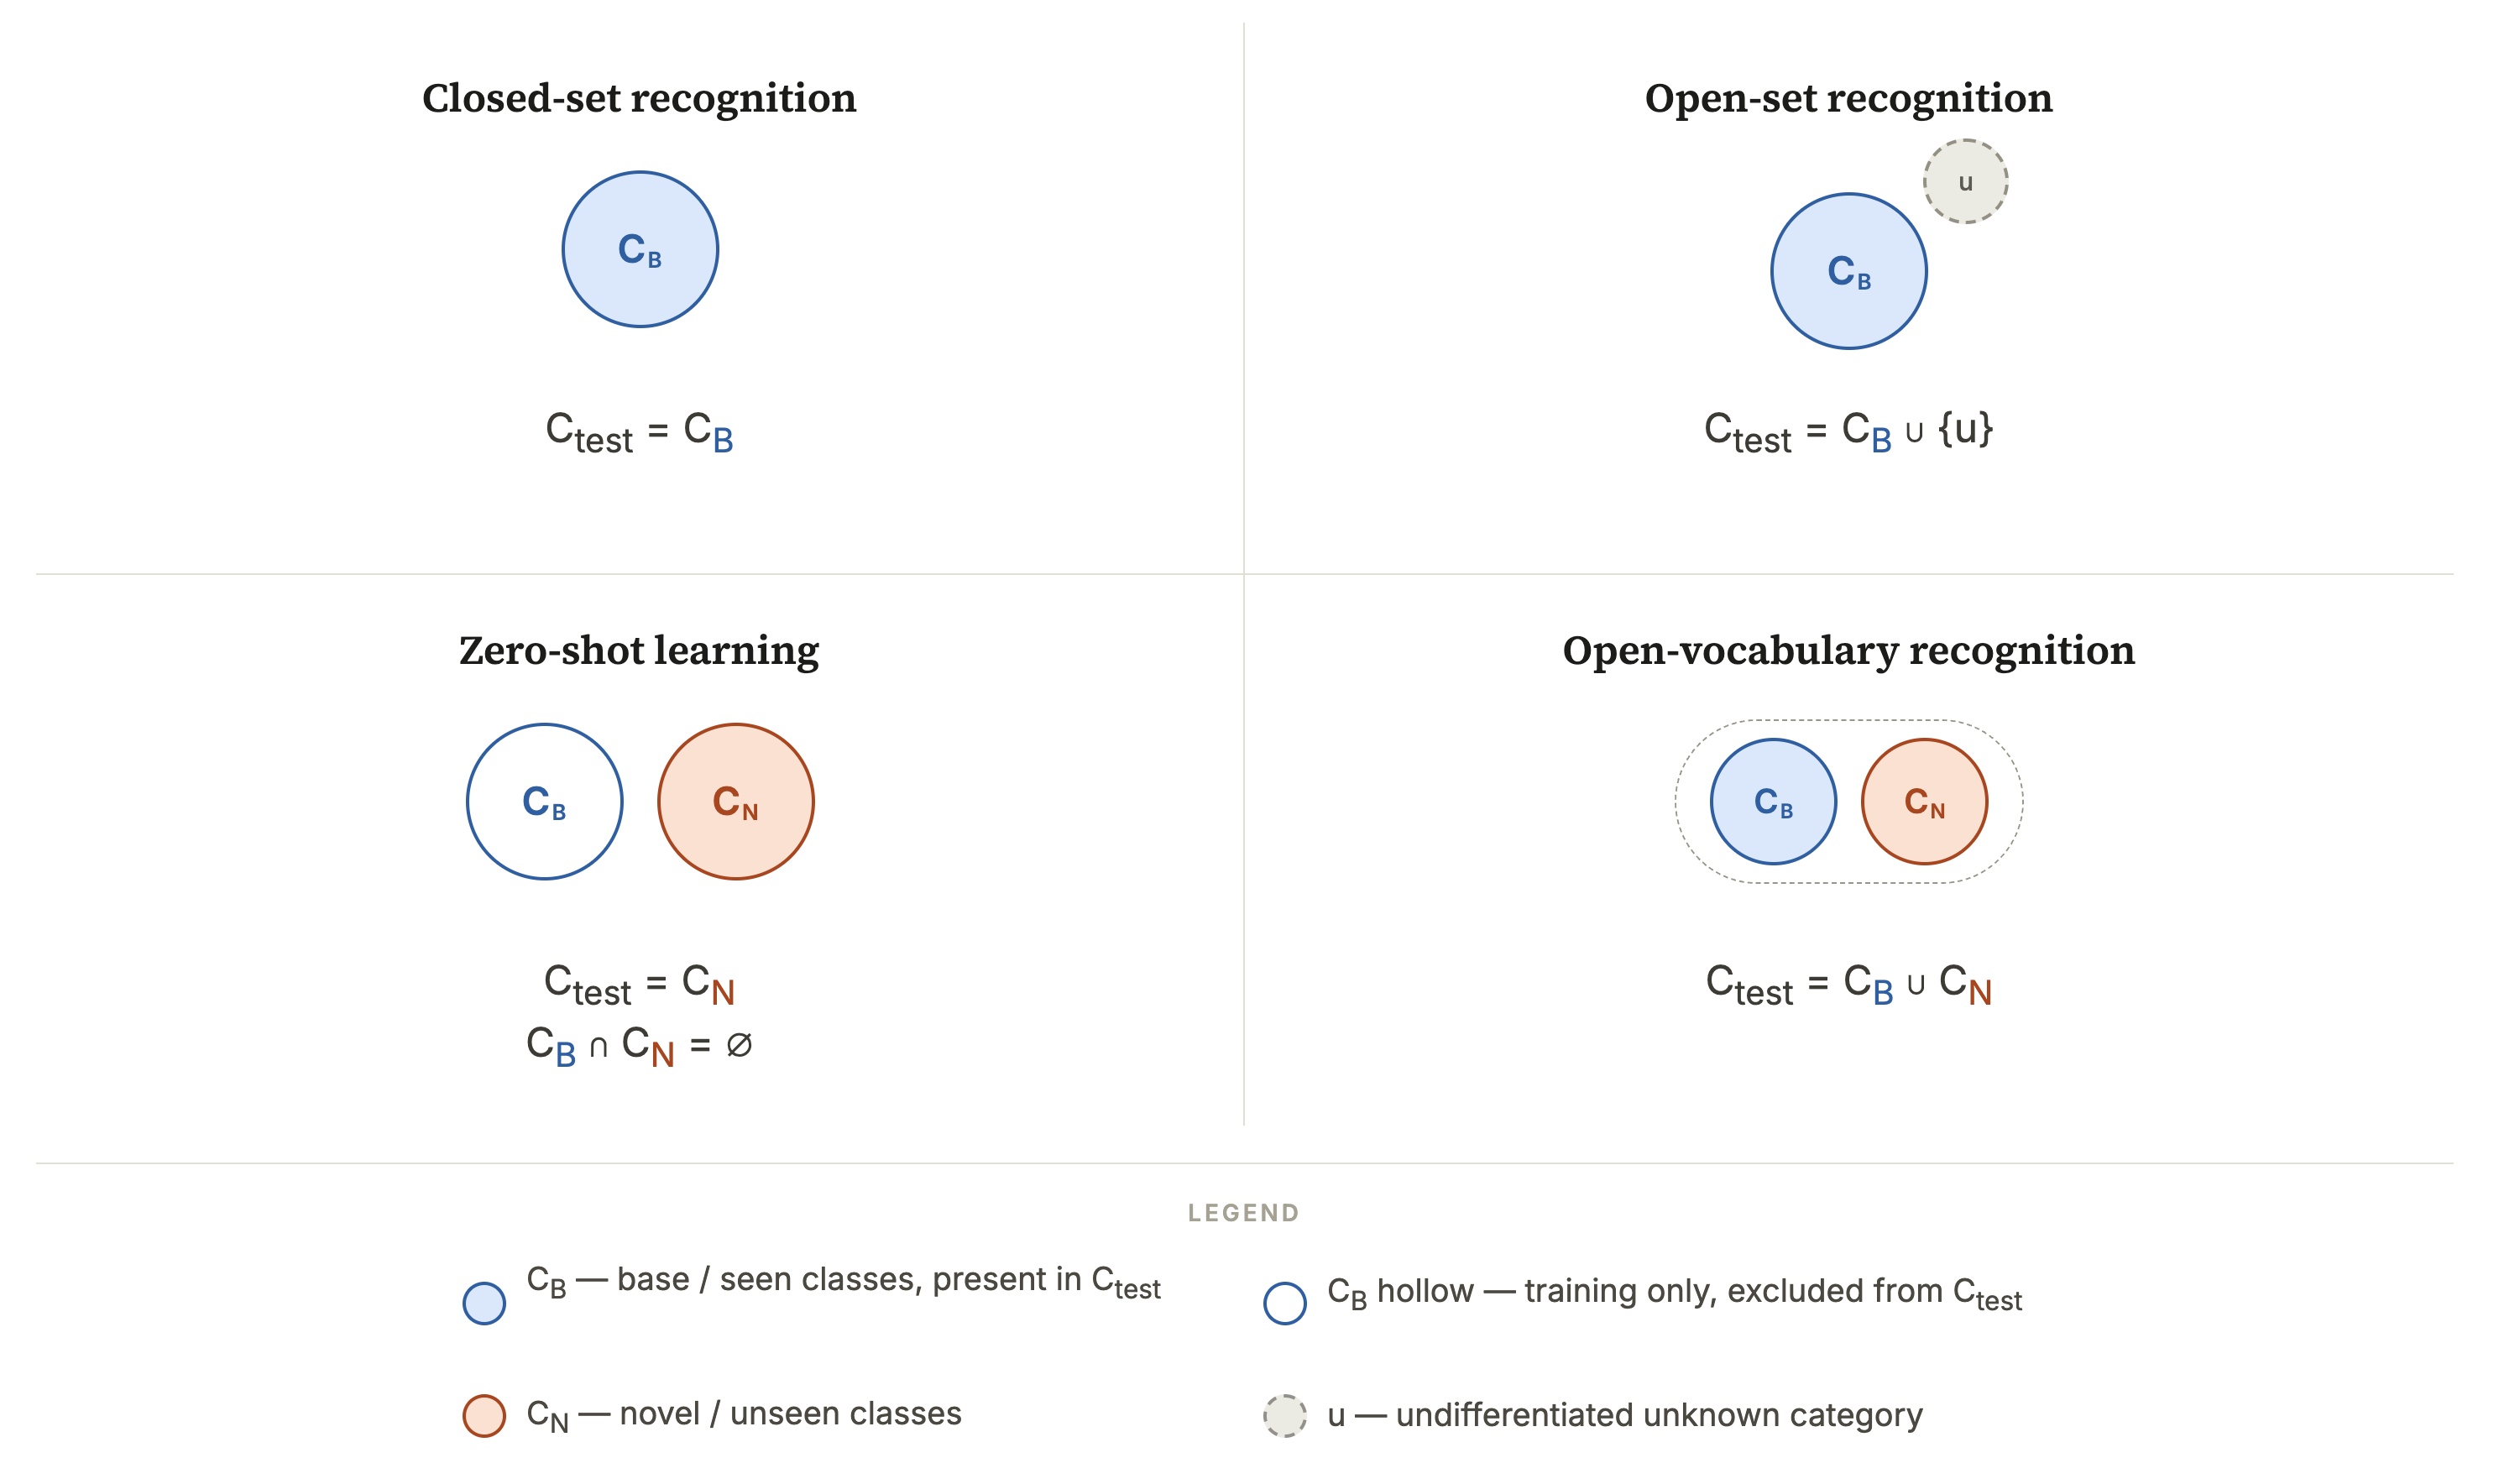
\includegraphics[width=\textwidth]{figures/cv_learning_paradigms_diagram.png}
  \caption{Label-space relationships for closed-set, open-set, zero-shot, and open-vocabulary recognition. \(C_B\), \(C_N\) and \(u\) denote base, novel, and unknown categories, respectively.}
  \label{fig:label-space-paradigms}
\end{figure}

\newpage
\noindent As summarised in Figure~\ref{fig:label-space-paradigms}, zero-shot and open-vocabulary learning are therefore related but distinct: zero-shot learning conventionally assumes a disjoint seen--unseen split and evaluates exclusively on \(C_N\), whereas open-vocabulary learning may draw on broader visual--language pretraining that is not constrained by this partition \cite{wu2024openvocabulary,zhu2024openvocabulary,cao2025zeroshot}. Modern open-vocabulary approaches commonly exploit image--text supervision or pretrained \glspl{VLM}, whose language-aligned representations provide semantic knowledge beyond the categories explicitly annotated in the task-specific training data \cite{wu2024openvocabulary,zhu2024openvocabulary}.

Large-scale pretraining has further enabled models to be transferred across downstream vision tasks and conditioned through prompts without conventional retraining \cite{reshadi2026deeplearningcv,Transformers4Vision}. \glspl{VLM} can use textual prompts to specify semantic concepts, while promptable segmentation models can use spatial prompts such as points or bounding boxes to specify regions of interest \cite{wu2024openvocabulary,BG38-segment-anything}. When such prompts are supplied only at inference time the pretrained model parameters remain unchanged, whereas fine-tuning instead updates model parameters using task-specific supervision \cite{BG38-segment-anything,reshadi2026deeplearningcv}.

\noindent Within detection, \emph{\gls{ZSD}} extends zero-shot learning by requiring both localisation and classification of objects belonging to categories that were not available as labelled classes during task-specific training \cite{cao2025zeroshot,zhu2024openvocabulary}. The broader experimental comparison in this dissertation is described as \emph{zero-shot localisation}, because the evaluated pretrained models may return bounding boxes, masks or other spatial predictions rather than conforming strictly to conventional \gls{ZSD} \cite{BG38-segment-anything,cao2025zeroshot}. A model is evaluated under this setting when it is applied to the \gls{MDWD} or \gls{MTSD} without labelled target-dataset training or task-specific parameter optimisation, while making no assumption that related concepts were absent from its original pretraining data \cite{wu2024openvocabulary,zhu2024openvocabulary,cao2025zeroshot}.

\subsection{Supervised Object Detection}
\label{sec:bg-supervised-od}
Supervised \gls{OD} learns to predict object categories and bounding boxes from annotated imagery, combining semantic classification with spatial localisation \cite{zou2023objectdetection}. In the conventional closed-set setting introduced in Subsection~\ref{sec:bg-cv-paradigms}, the detector is trained for a predefined set of labelled categories. This formulation requires substantial manually annotated training data, and performance can deteriorate when the deployment distribution differs from that represented during training \cite{zou2023objectdetection}. This dependence is particularly relevant to specialised domains: \citeauthor{robinson2026rfdetrneuralarchitecturesearch} report that detectors heavily optimised for \gls{COCO} can generalise poorly to real-world datasets with substantially different distributions, including differences in the number of objects per image, number of classes and dataset size \cite{robinson2026rfdetrneuralarchitecturesearch}.

\newpage
\noindent The development of \gls{DL}-based \gls{OD} has been shaped by a recurring trade-off between localisation accuracy, computational efficiency and deployment complexity \cite{zou2023objectdetection}. Region-based detectors established the two-stage paradigm by separating candidate-region generation from classification and bounding-box refinement \cite{girshick2014rcnn,girshick2015fastrcnn,ren2015faster}. Single-stage detectors instead perform localisation and classification directly from image features, substantially reducing inference cost and enabling real-time operation \cite{redmon2016you,liu2016ssd}. Transformer-based detectors introduced a further formulation based on direct set prediction, learned object queries and bipartite matching, reducing reliance on hand-designed components such as anchor boxes and \gls{NMS} \cite{carion2020end}. These families are reviewed below, followed by their application to waste and traffic-sign monitoring and the rationale for the detectors evaluated in this dissertation.

\subsubsection{Problem Formulation and Recurring Design Considerations}
\label{sec:bg-od-formulation}
Given an input image, a detector produces a set of predictions, each comprising a bounding box, a class label and a confidence score \cite{zou2023objectdetection}. During evaluation, predictions are matched to annotated \gls{GT} instances according to spatial overlap, commonly measured using \gls{IoU}, from which precision--recall curves and average-precision measures are derived \cite{lin2014coco}. Although this formulation is shared across detector families, architectures differ considerably in how candidate objects are represented, assigned during training and filtered during inference.

Central to this variation is label assignment, the process by which \gls{GT} objects are associated with candidate predictions during optimisation. Dense detectors generate predictions at many spatial locations and feature-map scales, requiring rules that determine which locations constitute positive training examples for each object \cite{zou2023objectdetection,tian2019fcos}. Earlier architectures relied on predefined anchor boxes of differing scales and aspect ratios, whereas anchor-free approaches predict object geometry directly from feature-map locations, removing anchor-specific hyperparameters that may be poorly matched to a new dataset \cite{tian2019fcos}. The assignment strategy is consequential because insufficient positive assignments impair localisation, particularly for small objects whose extent covers very few candidate locations.

Dense assignment strategies produce a high volume of predictions, giving rise to duplicate detections. Detection heads of this kind commonly produce several overlapping boxes for the same object and therefore employ \gls{NMS}, which ranks predictions by confidence and suppresses lower-confidence boxes whose overlap with a retained detection exceeds a threshold \cite{zou2023objectdetection}. Although effective, \gls{NMS} is a heuristic stage outside the learned model and may suppress legitimate neighbouring objects where instances occur in close proximity. End-to-end set-prediction detectors instead learn to produce one prediction per object directly, avoiding conventional duplicate suppression \cite{carion2020end, wang2024yolov10}.

\noindent These assignment and suppression mechanisms are further complicated by object scale, a persistent challenge in its own right. Street imagery contains objects ranging from large foreground instances to targets occupying only a few pixels. \Glspl{FPN} address this by combining semantically strong, low-resolution features with spatially precise, higher-resolution representations through top-down and lateral connections, allowing predictions at several resolutions rather than exclusively from the most heavily downsampled feature map \cite{lin2017fpn}. Small-object performance nevertheless remains substantially weaker than that for medium and large objects across many architectures, motivating the size-stratified reporting of average precision adopted by \gls{COCO} \cite{lin2014coco,zou2023objectdetection}.

\subsubsection{Two-Stage Region-Based Detectors}
\label{sec:bg-od-two-stage}
The \gls{R-CNN} family established the two-stage paradigm and dominated early \gls{DL}-based detection. \gls{R-CNN} itself generated class-agnostic candidate regions through selective search and processed each independently through a convolutional network before classification and box refinement, demonstrating the value of learned representations for localisation but at substantial computational redundancy \cite{girshick2014rcnn}. This redundancy was subsequently resolved by Fast \gls{R-CNN}, which computed convolutional features once per image and projected each proposal onto the shared feature map through \gls{RoI} pooling, enabling joint training of classification and regression \cite{girshick2015fastrcnn}. The remaining bottleneck of external region proposal was then eliminated by Faster \gls{R-CNN}, which integrated proposal generation directly into the network through a trainable \gls{RPN} sharing features with the detection head, establishing the characteristic two-stage structure of proposal followed by proposal-specific classification and refinement \cite{ren2015faster}. This progressive refinement gave two-stage systems strong localisation accuracy, further strengthened by integration with the \gls{FPN}, which fuses low-resolution semantic features with higher-resolution spatial detail across scales \cite{lin2017fpn,zou2023objectdetection}. The staged structure nevertheless introduces additional computation relative to direct prediction, a limitation that became increasingly consequential as detection expanded into video, autonomous systems and embedded applications where latency and throughput matter as much as benchmark accuracy \cite{redmon2016you,zou2023objectdetection}.

\subsubsection{Single-Stage Detectors}
\label{sec:bg-od-single-stage}
Single-stage detectors instead remove the explicit proposal-and-refinement separation and predict locations and categories directly from image features \cite{redmon2016you,liu2016ssd}. The original \gls{YOLO} treated detection as a unified regression problem, dividing the image into a grid and predicting boxes, objectness and class probabilities in a single network evaluation, yielding a substantial speed improvement at the cost of greater localisation error and weaker small-object performance \cite{redmon2016you}. \gls{SSD} adopted a comparable single-stage formulation but predicted from feature maps at several resolutions instead, so that smaller objects were represented by higher-resolution features and larger objects by deeper features with broader receptive fields \cite{liu2016ssd}. This multi-resolution design foreshadowed the multi-scale principle that became standard throughout later single-stage detectors.

Predicting densely across the entire image in this way, however, introduces an extreme imbalance between foreground objects and background candidate locations. RetinaNet identified this imbalance as a principal contributor to the historical accuracy gap between one- and two-stage detectors and introduced Focal Loss to down-weight easily classified examples, demonstrating that the gap arose partly from how dense predictions were supervised rather than from the single-stage formulation itself \cite{lin2017focal}. Combined with stronger backbones and improved assignment strategies, these developments progressively narrowed the separation between single- and two-stage performance \cite{zou2023objectdetection}. Single-stage architectures have consequently become prominent in deployment-oriented \gls{OD}, particularly where large image volumes must be processed under latency or hardware constraints. This balance is pertinent to municipal monitoring, where imagery may be acquired repeatedly from mobile or fixed platforms and where computational cost governs the practicality of large-scale deployment.

\subsubsection{The \gls{YOLO} Family}
\label{sec:bg-yolo}
The \gls{YOLO} family represents the principal lineage of single-stage real-time detection, and several generations illustrate the architectural changes that have progressively transformed it. \gls{YOLO}2 introduced anchor-based prediction, batch normalisation and multi-scale training, exposing an explicit speed--accuracy trade-off through variable input resolution \cite{redmon2017yolo9000}. \gls{YOLO}3 extended prediction across multiple feature scales using a deeper residual backbone \cite{redmon2018yolov3}. \gls{YOLO}4 combined cross-stage partial connections, path aggregation and extensive augmentation to improve accuracy while preserving real-time inference \cite{bochkovskiy2020yolov4}. \gls{YOLO}7 introduced Extended Efficient Layer Aggregation Networks and training-time refinements that add no inference cost \cite{wang2023yolov7}, while \gls{YOLO}9 proposed Programmable Gradient Information to mitigate information loss in deep detector architectures \cite{wang2024yolov9}.

A more substantial change appeared with \gls{YOLO}10, which introduced consistent dual label assignment, whereby a one-to-many head provides rich supervision during training while a one-to-one head supports non-redundant predictions so that inference no longer requires \gls{NMS} \cite{wang2024yolov10}. This development substantially narrowed the distinction that had previously separated dense \gls{YOLO}-style detectors from the set-prediction formulation used by Transformer-based detectors such as \gls{DETR}.

\newpage
\noindent The recent generations leading to the models evaluated in this dissertation illustrate materially different architectural emphases. \gls{YOLO}11 retains a predominantly convolutional backbone--neck--head structure while introducing compact C3k2 blocks and the C2PSA attention module to strengthen spatial feature modelling, with an anchor-free head available across several capacity scales \cite{yolo11}. \gls{YOLO}12 moves the lineage towards attention-centric feature modelling through Area Attention, which partitions attention computation to retain a broad receptive field at reduced cost, and Residual Efficient Layer Aggregation Networks for stable optimisation \cite{tian2025yolov12}. It integrates attention more centrally into the representation without becoming a conventional \gls{VIT}, preserving the real-time latency characteristic of \gls{YOLO} detectors while adopting the attention-based feature modelling associated with Transformer architectures.

\gls{YOLO}26 shifts emphasis towards native end-to-end and edge-oriented inference, whereby a dual-head design yields \gls{NMS}-free one-to-one predictions, with the one-to-many head used only during training, while Distribution Focal Loss is removed to simplify the inference graph \cite{jocher2026yolo26}. Its training procedure is adapted accordingly, with Small-Target-Aware Label Assignment improving positive-sample coverage for objects spanning few candidate locations, Progressive Loss stabilising optimisation as reliance shifts towards the one-to-one head, and the \gls{MuSGD} optimiser supporting convergence under this dual-head regime \cite{jocher2026yolo26}. These developments are directly pertinent to small targets and constrained hardware, although architectural simplification does not guarantee superior accuracy or latency on every dataset.

\subsubsection{Transformer-Based Detection}
\label{sec:bg-transformer-detection}
\gls{DETR} introduced a distinct formulation of \gls{OD} based on direct set prediction, departing entirely from the region-proposal and dense-anchor mechanisms underlying earlier detectors \cite{carion2020end}. An image representation extracted by a convolutional backbone is passed through a Transformer encoder, which models relationships across the feature map and, in doing so, makes contextual information from spatially distant regions available during subsequent query refinement. A decoder then attends over a fixed set of learned object queries, each of which is refined into a class prediction and bounding box, with one-to-one bipartite matching during training encouraging every \gls{GT} instance to be represented by exactly one prediction and thereby removing the need for anchors and \gls{NMS} \cite{carion2020end,yu2025detrreview}.

The original \gls{DETR} nevertheless converged slowly, imposed considerable computational cost through global self-attention on high-resolution features, and performed comparatively weakly on small objects \cite{carion2020end,yu2025detrreview}. Deformable \gls{DETR} addressed these limitations by sampling a small set of learned locations around reference points across several feature resolutions rather than attending densely over every position, a multi-scale deformable attention mechanism that reduced cost, accelerated convergence and gave higher-resolution features direct influence on query refinement \cite{zhu2021deformabledetr}.

\gls{RT-DETR} subsequently adapted this Transformer-based formulation to real-time constraints through a hybrid encoder that separates intra-scale interaction from cross-scale fusion, avoiding indiscriminate Transformer processing across all feature levels, together with uncertainty-minimal query selection that initialises object queries from high-quality encoder features \cite{zhao2024rtdetr}. The resulting detector demonstrated that an end-to-end, \gls{NMS}-free Transformer could compete directly with real-time \gls{YOLO} models in both accuracy and latency \cite{zhao2024rtdetr}. The contrast between contemporary convolutional and Transformer-based detectors is therefore more nuanced than the historical division between fast single-stage and accurate but expensive alternatives. Both now incorporate multi-scale representation, sophisticated assignment and end-to-end prediction, and their remaining differences concern how spatial context is modelled, how candidate objects are represented, the computational profile of extractor and decoder, and their behaviour under dataset-specific conditions such as small targets, clutter and densely positioned instances \cite{yu2025detrreview}.

\glsreset{RF-DETR}
\subsubsection{The \gls{RF-DETR} Model}
\label{sec:bg-rfdetr}
\gls{RF-DETR} is a recent real-time end-to-end detector that develops the \gls{DETR} lineage by combining query-based detection with large-scale self-supervised pretraining and architecture optimisation \cite{robinson2026rfdetrneuralarchitecturesearch}. Building upon \gls{LW-DETR}, it replaces the backbone with a pretrained \gls{DINO}v2 \gls{VIT}, so that detection begins from representations learnt through large-scale self-supervision rather than solely from the target dataset, while retaining multi-scale features supplied to a query-based decoder, one-to-one matching during training and \gls{NMS}-free inference \cite{robinson2026rfdetrneuralarchitecturesearch}. This design is motivated by \citeauthor{robinson2026rfdetrneuralarchitecturesearch}'s observation that architectures and training procedures heavily optimised for \gls{COCO} do not necessarily retain their performance on datasets with different numbers of objects, categories and examples \cite{robinson2026rfdetrneuralarchitecturesearch}.

Beyond its backbone and query-based decoding, \gls{RF-DETR} additionally employs \gls{NAS}, which automates the discovery of architectural configurations by searching over structural choices rather than fixing them by hand. Its weight-sharing variant allows candidate configurations to share a single set of trained weights during the search, substantially reducing the cost of exploring the accuracy--latency trade-off \cite{robinson2026rfdetrneuralarchitecturesearch}. The search varies input resolution, patch size, decoder depth, query count and the number of windows per attention block within this shared framework, yielding a family of configurations that occupy different operating points rather than uniformly scaled replicas. Consequently, the nominal size labels assigned to \gls{RF-DETR} variants do not correspond to equally named \gls{YOLO} models in parameter count, resolution or capacity, a distinction considered explicitly in the model-scale comparisons of Subsection~\ref{sec:supervised-model-ablation}.

\subsubsection{Supervised Detection in Municipal Monitoring}
\label{sec:bg-od-municipal}
Municipal monitoring places supervised \gls{OD} in substantially less controlled conditions than many conventional recognition tasks. Waste may vary considerably in shape, material and appearance and often occurs in cluttered or overlapping arrangements, whereas traffic signs are visually more structured but frequently occupy only a small proportion of the image and are affected by distance, occlusion and illumination \cite{BG17-small-signs,BG20-sign-glare}. These differences make detector selection dependent not only on predictive accuracy, but also on how well an architecture handles the visual characteristics and computational requirements of the target domain.

The \gls{YOLO} family has consequently been prominent in applied municipal-monitoring research, particularly where repeated image processing favours low-latency inference. In waste monitoring, \citeauthor{decarolis2020yolotrashnet} developed YOLO TrashNet from \gls{YOLO}3 for the detection and reporting of abandoned waste \cite{decarolis2020yolotrashnet}, demonstrating an early use of \gls{OD} within an operational reporting workflow. More recently, \gls{YOLO}8, \gls{YOLO}9 and \gls{YOLO}10 were compared on pLitterStreet before the selected detector was applied to Google Street View imagery for spatial litter mapping \cite{espinosa2025litter}, and \gls{YOLO}11 was used to detect both garbage and potholes within a municipal reporting workflow \cite{reddy2025yologarbagepothole}. These studies illustrate a shift from recognising waste in isolation towards using detections as spatial observations of street-level conditions.

A similar emphasis on efficient detection is evident in traffic-sign research, although the small image-space extent of signs has encouraged greater attention to feature preservation and multi-scale representation. A series of modifications to \gls{YOLO}5 and \gls{YOLO}7 introduced coordinate, channel and spatial attention, dynamic label assignment and multi-scale feature fusion specifically to improve small-sign detection under complex road conditions \cite{wang2023improvedtrafficsign,shi2023scyolo,mahadshetti2024signyolo}, while \citeauthor{liu2024yolots} developed YOLO-TS from \gls{YOLO}8n to reduce computational demand while retaining performance on small traffic signs \cite{liu2024yolots}. Across this work, small-target representation, feature fusion, attention and deployment cost are treated as interdependent design considerations rather than accuracy in isolation.

Transformer-based detectors provide a contrasting approach through query-based set prediction and attention-based feature modelling. Recent traffic-sign studies suggest that these architectures can also operate within real-time constraints when adapted to the domain. \citeauthor{lin2025tsdetr} proposed TS-DETR, combining positive- and negative-sample augmentation with multi-scale feature integration to address small targets and class imbalance \cite{lin2025tsdetr}, while \citeauthor{dong2026hasdetr} adapted \gls{RT-DETR} through HAS-DETR, introducing high-frequency feature preservation, cross-scale fusion and a dedicated small-target enhancement head \cite{dong2026hasdetr}. Both studies retain the end-to-end Transformer formulation while explicitly modifying it around the characteristics of traffic-sign imagery. Early infrastructure studies have also begun to evaluate \gls{RF-DETR} directly against \gls{YOLO} for road-surface and road-damage assessment \cite{kurrey2026roadsurface,amores2026roaddamage}, although its application base remains considerably smaller than that of either \gls{YOLO} or \gls{RT-DETR}.

More direct comparisons indicate that neither detector family is uniformly preferable. \citeauthor{kumar2026gvp} compared \gls{YOLO}8, \gls{YOLO}10, \gls{YOLO}11m and \gls{RT-DETR} for monitoring garbage-vulnerable points using a street-side camera and \gls{IoT} infrastructure \cite{kumar2026gvp}. The system coupled detection with temporal analysis of dumping and cleaning activity, placing the comparison within an operational waste-monitoring setting rather than an isolated benchmark. In traffic-sign condition assessment, \gls{YOLO}11 and \gls{RT-DETR} were compared for detecting fading and delamination from vehicle-acquired roadway imagery \cite{pandey2026signcondition}. Relative performance depended on the defect: \gls{YOLO}11 performed better for fading and achieved lower end-to-end runtime, whereas \gls{RT-DETR} showed a smaller advantage for delamination. This suggests that architectural preference can vary even within the same municipal asset class.

\subsubsection{Selection of Detection Architectures}
\label{sec:bg-selection-od}
Taken together, the literature indicates that detector performance is strongly dependent on the visual and operational characteristics of the target domain. Waste monitoring involves irregular object geometry, heterogeneous appearance, clutter and frequent co-occurrence, whereas traffic-sign monitoring places greater emphasis on small-object localisation, viewing distance, illumination and, where condition is considered, subtle degradation cues. Performance reported on generic benchmarks, or within one municipal domain, therefore cannot be assumed to transfer directly to another \cite{robinson2026rfdetrneuralarchitecturesearch,pandey2026signcondition}.

The detectors evaluated in this dissertation were selected to examine these differences across two contemporary real-time detection lineages. \gls{YOLO}11, \gls{YOLO}12 and \gls{YOLO}26 represent recent stages in the development of the single-stage family, spanning predominantly convolutional feature modelling, more attention-centric representations and native end-to-end prediction \cite{yolo11,tian2025yolov12,jocher2026yolo26}. \gls{RF-DETR} provides a Transformer-based counterpart operating within the same real-time setting, but differs through query-based prediction, a self-supervised pretrained backbone and architecture-search-based scaling \cite{robinson2026rfdetrneuralarchitecturesearch}. Rather than assuming that either lineage will transfer uniformly across domains, all detectors are evaluated under a common protocol on both datasets, as described in Section~\ref{sec:supervised-detection-methodology}.

\subsection{Zero-Shot and Prompt-Based Object Localisation}
\label{sec:bg-zero-shot}
The development of large-scale pretrained visual models has broadened the means by which localisation tasks can be specified beyond the fixed category spaces associated with conventional supervised \gls{OD}. Rather than learning every target category exclusively from task-specific bounding-box annotations, contemporary approaches increasingly exploit visual representations acquired from large and heterogeneous datasets, with the target concept supplied through language, visual exemplars or spatial prompts at inference time \cite{bommasani2021opportunities,radford2021learning,xiao2024florence2}. This progression has produced several related but architecturally distinct approaches, including open-vocabulary detection, promptable segmentation and grounded \glspl{VLM}. Their principal attraction lies in the ability to transfer pretrained capabilities to new concepts with little or no target-domain supervision, although this flexibility remains dependent on the correspondence between the target domain, the pretraining distribution and the prompts used to specify the task.

\subsubsection{Foundation Models and Zero-Shot Visual Transfer}
\label{sec:bg-foundation-models}
The concept of a \gls{FM} describes a model pretrained at scale on broad data and subsequently transferable across a range of downstream tasks rather than optimised exclusively for a single predefined objective \cite{bommasani2021opportunities}. In \gls{CV}, an important development towards this formulation was the use of natural-language supervision to replace or complement manually defined class vocabularies. Radford et al.~\cite{radford2021learning}, for example, trained \gls{CLIP} contrastively on 400 million image--text pairs, learning a shared representation in which visual concepts could subsequently be referenced through natural language. This enabled zero-shot transfer across a diverse collection of recognition tasks without dataset-specific parameter optimisation and established image--language pretraining as a practical mechanism for transferring visual knowledge beyond a fixed training taxonomy.

Large-scale pretraining does not, however, remove the distinction between zero-shot, few-shot and supervised adaptation. As defined in Subsection~\ref{sec:bg-cv-paradigms}, zero-shot inference applies the pretrained capability without updating model parameters on the target dataset, whereas few-shot methods introduce a limited amount of target-specific evidence through examples or restricted adaptation. Fully supervised approaches make substantially greater use of labelled target data and consequently offer greater opportunity for specialisation. The trade-off is therefore between adaptability and target-domain optimisation: zero-shot systems reduce annotation and retraining requirements but remain constrained by what their pretrained representations encode, while supervised models can learn distinctions that are specific to a local taxonomy or visual environment.

The experiments reported by Radford et al.~\cite{radford2021learning} illustrate that this relationship is not simply monotonic with the number of labelled examples. Their zero-shot formulation was competitive with low-shot linear probing in several settings, while the authors also observed that language alone remains inadequate for visual concepts that are difficult to express textually and that supervised performance remained stronger on many datasets. Zero-shot capability should therefore be understood as a transfer property rather than an assumption of equivalent performance to task-specific supervision.

Subsequent \glspl{FM} have extended this principle beyond image-level recognition towards multiple spatial and semantic tasks. Florence-2, for example, adopts a unified sequence-to-sequence architecture in which textual task prompts can elicit captioning, detection, grounding or segmentation outputs from the same model \cite{xiao2024florence2}. Its pretraining corpus contains 5.4 billion annotations across 126 million images spanning image-, region- and pixel-level supervision. This progression is important because it shifts the role of prompting from selecting among image-level semantic categories towards specifying both the visual concept and the form of spatial information required from the model.

\subsubsection{Promptable Segmentation and the Segment Anything Family}
\label{sec:bg-sam}

A parallel development occurred in segmentation through the introduction of promptable visual segmentation. The original \gls{SAM} separated image encoding from prompt-conditioned mask prediction, allowing a target region to be specified using spatial cues such as points or bounding boxes rather than through a fixed semantic category \cite{kirillov2023segment}. \gls{SAM}~2 extended this formulation from static images to video through a memory-based architecture capable of propagating and refining prompted objects across frames while retaining the point-, box- and mask-based interaction of the original model \cite{ravi2024sam2}. The principal capability of these models was therefore spatial generalisation: they could delineate previously unseen objects when supplied with an indication of which object should be segmented, but the prompt itself did not necessarily communicate semantic identity.

This distinction motivated combinations of promptable segmentation with language-grounded detection. Grounded SAM, for example, couples Grounding DINO with \gls{SAM}, using a textual query to identify corresponding regions before supplying the resulting boxes to the segmentation model \cite{ren2024grounded}. The resulting pipeline combines semantic flexibility with pixel-level localisation without requiring the segmentation component itself to perform open-vocabulary recognition.

\gls{SAM}~3 subsequently integrates semantic concept prompting more directly into the Segment Anything formulation. Rather than requiring the location of an individual instance to be provided in advance, the model introduces promptable concept segmentation, in which short noun phrases, image exemplars or combinations of the two can be used to detect and segment all matching instances within an image or video \cite{meta2025sam3}. Positive and negative exemplars can additionally refine the intended concept, providing a form of visual few-shot specification alongside language prompting. This broader capability also introduces semantic ambiguity absent from purely spatial prompting, since noun phrases may admit multiple visual interpretations and their correspondence can be affected by occlusion, blur or subjective descriptors. Prompt formulation and exemplar selection therefore become part of the effective task definition rather than merely an interface choice.

\subsubsection{Open-Vocabulary and Language-Grounded Localisation}
\label{sec:bg-open-vocabulary}

The development of open-vocabulary localisation similarly reflects the movement from image-level language alignment towards region-level grounding. While models such as \gls{CLIP} demonstrated that visual representations could be associated with arbitrary textual concepts, image-level contrastive supervision does not itself establish where those concepts occur within an image \cite{radford2021learning}. Open-vocabulary detection addresses this limitation by explicitly aligning textual representations with spatial image regions, allowing language to specify the objects to be localised.

Grounding DINO represents a prominent development of this formulation by integrating grounded language supervision with a Transformer-based detector \cite{liu2024grounding}. Rather than attaching language only to the final classification stage, the architecture introduces cross-modal interaction during feature enhancement, query selection and decoding, enabling categories and referring expressions to influence the localisation process throughout the network. The model can consequently detect objects specified through category names or descriptive expressions without requiring the corresponding target dataset to have been used for task-specific training.

This flexibility differentiates grounded localisation from conventional closed-set \gls{OD}, where adding a new semantic category generally requires additional labelled examples and model adaptation. It also differs from the earlier Segment Anything formulation, in which the prompt primarily identifies \emph{where} the target object lies rather than \emph{what} concept should be found. Language-grounded localisation must infer both simultaneously, increasing semantic flexibility but also introducing sensitivity to terminology. This is particularly relevant to specialised monitoring taxonomies, where an operational category may be visually meaningful within a local context while differing from the language and concepts represented during large-scale pretraining.

\subsubsection{Locate Anything}
\label{sec:bg-locate-anything}

The extension of language grounding into generative \glspl{VLM} has introduced a further localisation formulation in which spatial coordinates are represented within the model's output sequence. Conventional generative grounding commonly serialises a bounding box into several coordinate tokens that are decoded sequentially, allowing spatial prediction to share the same general interface as textual generation but imposing both computational and structural limitations when numerous objects must be returned \cite{nvidia2026locateanything}.

LocateAnything addresses this limitation through Parallel Box Decoding, treating geometric entities such as bounding boxes and points as coupled spatial units rather than independent tokens \cite{nvidia2026locateanything}. Its large-scale grounding framework is trained on more than 138 million localisation samples and supports multiple forms of visual grounding and detection within a common vision--language architecture. By decoding the coordinates belonging to a geometric unit in parallel, the model seeks to preserve their spatial relationship while reducing the sequential inference cost associated with autoregressive coordinate generation.

This formulation is particularly relevant to comparisons with conventional \gls{OD} because it produces explicit spatial predictions while retaining the semantic flexibility of a generative \gls{VLM}. The distinction nevertheless remains important: localisation is generated through a vision--language decoding process rather than a conventional detector head, so its output structure, confidence information and inference behaviour need not correspond directly to those of supervised detectors. The LocateAnything study additionally considers dense and overlapping scenes, where maintaining separation between adjacent predictions is especially demanding, making the approach relevant to localisation problems containing multiple closely positioned instances.

\subsubsection{Vision--Language Models and Grounded Visual Reasoning}
\label{sec:bg-vlm-grounding}

Grounded \glspl{VLM} generalise this formulation further by combining visual localisation with the broader language-generation capabilities of multimodal models. Whereas a dedicated detector is principally optimised to produce categories, locations and confidence scores, a \gls{VLM} can place spatial predictions within a richer generated response that also describes objects, relationships or contextual properties. Florence-2 demonstrates an intermediate form of this unification, using textual task prompts and a shared sequence representation for detection, grounding, segmentation and language-based visual understanding \cite{xiao2024florence2}, while more recent generative grounding models incorporate coordinates directly into multimodal output sequences \cite{nvidia2026locateanything}.

The broader output space provides greater flexibility but creates additional reliability requirements. Spatial predictions must remain geometrically valid and complete while the generated semantic interpretation must remain grounded in the visual evidence. Recent evaluation of multimodal language models has shown that linguistically plausible outputs do not necessarily imply faithful visual grounding, with errors arising from target-region binding, transcription and language-prior effects even where the visual evidence is comparatively clear \cite{wang2026symbolconsistency}. Such behaviour is particularly relevant to roadside imagery containing text, symbols or multiple similar objects, since a plausible semantic response may still refer to the wrong visual instance.

Grounded \glspl{VLM} should therefore be distinguished from specialised localisation architectures despite their ability to emit bounding boxes or points. Their advantage lies in combining localisation with semantic and contextual interpretation, while their broader generative formulation introduces additional opportunities for omission, spatial inconsistency and visually unsupported output. Whether this additional flexibility provides practical value consequently depends on the extent to which the monitoring task requires reasoning beyond object presence and location.

\subsubsection{World Foundation Models and the NVIDIA Cosmos Family}
\label{sec:bg-cosmos}

\Glspl{WFM} broaden the scope of foundation modelling from static visual recognition towards representations of physical environments and their evolution over time. NVIDIA's Cosmos platform defines a \gls{WFM} as a broadly pretrained world model that can subsequently be specialised for downstream physical-\gls{AI} applications, using large-scale video data to acquire general representations of visual dynamics before post-training for particular environments or tasks \cite{nvidia2025cosmosplatform}. This differs from conventional \gls{OD} and visual grounding because the intended representation encompasses not only object identity and location but also temporal behaviour and physical interaction.

Cosmos-Reason1 develops the reasoning component of this formulation through multimodal models trained to interpret video using representations of physical common sense and embodied reasoning \cite{nvidia2025cosmosreason1}. Its emphasis lies on spatial, temporal and physical relationships and on producing reasoned natural-language responses or embodied decisions, rather than on replacing a dedicated object detector. The Cosmos Reason2 models evaluated in this dissertation are reasoning \glspl{VLM} from this family, applied here to static images and bounding-box generation rather than video prediction or action generation \cite{nvidia2025cosmosreason2}. Cosmos~3 subsequently extends the family towards an omnimodal architecture capable of jointly processing and generating language, images, video, audio and action sequences, thereby integrating visual understanding, generation and action modelling within a common framework \cite{nvidia2026cosmos3}.

For municipal visual monitoring, the relevance of this broader modelling direction lies in the distinction between recognising an object and interpreting its context. A dedicated detector may establish that waste or a traffic sign is present, whereas a physically grounded model may potentially reason about temporal persistence, spatial relationships or the surrounding scene. The literature supporting these models is, however, presently concentrated primarily on general visual grounding, robotics, autonomous systems and embodied \gls{AI}, rather than on municipal inspection itself. Their applicability to street-level waste and infrastructure monitoring therefore remains an empirical question rather than an established result.

Taken together, the literature reflects a progression from representations learned for fixed visual categories towards increasingly general systems in which the required concept, location or task can be communicated at inference time. Image--language pretraining first provided the semantic basis for zero-shot transfer, open-vocabulary detectors extended this alignment to spatial regions, promptable segmentation introduced flexible object delineation, and grounded \glspl{VLM} increasingly combine localisation with generated semantic or contextual interpretation. These approaches reduce dependence on task-specific annotation and make the queried vocabulary substantially more adaptable, but they do not eliminate the effects of domain shift, semantic ambiguity or prompt sensitivity. Their evaluation alongside supervised \gls{OD} on the \gls{MDWD} and \gls{MTSD} therefore provides a means of examining whether this increased flexibility can be realised without unacceptable losses in localisation reliability under municipal street-level conditions.



\subsection{Visual Representation Learning for Attribute Classification}
\label{sec:bg-representation}

    \subsubsection{Transfer Learning and Visual Representation Learning}
    \label{sec:bg-transfer-learning}

    \subsubsection{Self-Supervised Visual Representation Learning}
    \label{sec:bg-self-supervised}

    \subsubsection{DINOv3}
    \label{sec:bg-dinov3}

    \subsubsection{V-JEPA 2.1}
    \label{sec:bg-vjepa}

    \subsubsection{Supervised and Vision--Language Representations}
    \label{sec:bg-representation-baselines}

    \subsubsection{Adapting Pretrained Representations}
    \label{sec:bg-transfer-strategies}

    \subsubsection{Multi-Attribute Classification}
    \label{sec:bg-multiattribute}


\section{Deployment and Evaluation Considerations}
\label{sec:bg-deployment-evaluation}

\subsection{Deployment Architectures for Municipal Visual Monitoring}
\label{sec:bg-deployment}

    \subsubsection{Cloud, Edge and On-Device Computing}
    \label{sec:bg-edge}

    \subsubsection{Computational Efficiency and Deployment Constraints}
    \label{sec:bg-computational-efficiency}

\subsection{Evaluation Considerations for Visual Monitoring Systems}
\label{sec:bg-evaluation}

    \subsubsection{Robustness and Failure Analysis}
    \label{sec:bg-robustness}

    \subsubsection{Deployment-Oriented Evaluation}
    \label{sec:bg-deployment-evaluation-metrics}

\noindent\rule{\linewidth}{0.3pt}